\documentclass[../../main/main.tex]{subfiles}

\begin{document}
\chapter{22/09/2020}
\label{cpt:lec1}

\section{Introduction}
\label{sec:introduction}

Our aim is to abstract and generalize concepts such as {\bf space}, {\bf distance} and {\bf continuity}.

As en example of the character of this theory, we intend not to distinguish subspaces A (circle) and B (square) of $\mathbb{R}^{2}$, but to distinguish these from C (ring), as in figure \ref{fig:example-1}.

\begin{figure}[ht]
  \centering
  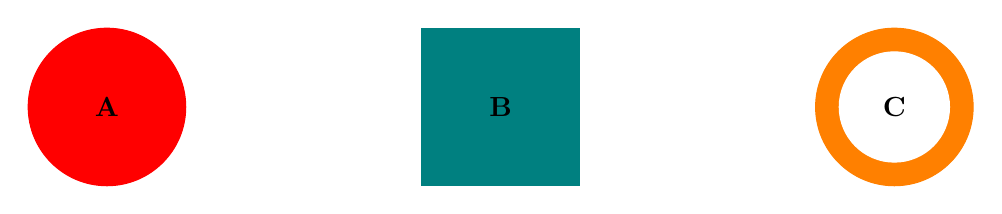
\begin{tikzpicture}
    \draw [fill=red, red] (-5, 0) circle [radius=1];
    \draw [fill= teal, teal] (-1, -1) rectangle (1, 1);
    \draw [fill=orange, orange] (5, 0) circle [radius=1];
    \draw [fill=white, white] (5, 0) circle [radius=.7];
    \node at (-5, 0) {{\bf A}};
    \node at (0, 0) {{\bf B}};
    \node at (5, 0) {{\bf C}};
  \end{tikzpicture}
  \caption{Examples of topological subspaces of $\mathbb{R}^{2}$.}
  \label{fig:example-1}
\end{figure}

\section{Topological Spaces}
\label{sec:top-spaces}

\begin{definition}
  Given a set $X$, we denote the the set of all subsets of $X$ as $\mathcal{P}(X)$, called the {\bf power set} of $X$.
\end{definition}

In topology, the union of potentially infinite (and uncountable) subsets. We write the union of a family of subsets $\{A_{i} : i \in I\}$ as $\cup_{i \in I} A_{i}$.

\begin{definition}
  \label{def:topology}
  Given a non-empty set $X$, we say $\Top \subseteq \mathcal{P}(X)$ is a {\bf topology} on $X$ if:
  \begin{enumerate}
      \item $X, \emptyset \in \Top$
      \item if $A, B \in \Top$ then $A \cap B \in \Top$
      \item if $A_{i} \in \Top$ for all $i \in I$, then $\bigcup_{i \in I} A_{i} \in \Top$.
  \end{enumerate}
  Then $(X, \Top)$ is a {\bf topological space}, and the elements of $X$ sometimes denotes by points.
\end{definition}

\begin{remark}
  For a finite family of subsets $N$, the reunion $\bigcap_{i \in N} A_{i} \in \Top$.
\end{remark}
\begin{proof}
  The case for $n = 2$ is taken care by the second axiom in \ref{def:topology}. Assume $\bigcap_{i=1}^{n} A_{i} = B \in \Top$. Then
  \begin{equation*}
    \bigcap_{i=1}^{n+1} A_{i} = \left(  \bigcap_{i=1}^{n} A_{i} \right) \cap A_{n+1} = B \cap A \in \Top
  \end{equation*}
  so the statement holds by induction.
\end{proof}

\begin{example}
  Let $X_{1} = \left\{ a, b, c, d, e, f \right\}$ and $\Top_{1} = \left\{ X_{1}, \emptyset, \{a\}, \{c, b\}, \{a, c, d\}, \{b, c, d, e, f\} \right\}$. Then $\Top_{1}$ is a topology on $X_{1}$.
\end{example}

\begin{remark}
  For a finite set $X$, one does enough to test the union of each two subsets of $\Top$, and the finite union follows by induction.
\end{remark}

\begin{example}
  Let $X = \{a, b, c, d\}$ and $\Top_{2} = \left\{ X_{2}, \emptyset, \{a\}, \{c, d\}, \{a, c\}, \{a, c, d\} \right\}$. Then $\Top_{2}$ is not a topology on $X_{2}$, for $\{a\} \cap \{a, c\} = \{c\} \notin \Top$.
\end{example}

\begin{example}
  Let $\Top_{3} \subseteq \mathcal{P}(\mathbb{N})$ be such that
  \begin{equation*}
    \Top_{3} = \{\mathbb{N}\} \cup \left\{ A \subseteq \mathbb{N} : A \text{ is finite} \right\}.
  \end{equation*}
  $\Top_{3}$ is not a topology on $\mathbb{N}$. Let $B_{n} = \{2 n + 1\}$ for $n \in \mathbb{N}$. Then $B_{n} \in \Top_{3}$ but
  \begin{equation*}
    \bigcup_{n = 1}^{\infty} B_{n} \notin \Top_{3}.
  \end{equation*}
\end{example}

\begin{definition}
  \label{def:discrete-topology}
  Let  $X$ be a non-empty set. Then $\Top = \mathcal{P}(X)$ is a topology on $X$, called the {\bf discrete topology}.
\end{definition}

\begin{remark}
  Let $(X, \Top)$ be a topological space. Then $\Top$ is the discrete topology if and only if $\{x\} \in \Top$ for all $x \in X$. These are called the {\bf singular sets} of $X$.
\end{remark}
\begin{proof}
  Take $A \in \mathcal{P}(X)$ and let $x_{i}$ for $i \in I$ be elements of $X$. If $A$ is empty then it is simply the {\bf empty union} of singleton sets. Otherwise, it implies that there does not exist a union such that
  \begin{equation*}
    \bigcup_{i \in I} \{x_{i}\} = A.
  \end{equation*}
  Then there exists an element $x_{k} \in A$ that is not contained in the union. As every element of $X$ is contained in the union of singletons sets of $X$, $A$ contains an element that is not contained in $X$. Hence $A \notin \mathcal{P}(X)$, which is contradiction.
\end{proof}

\begin{definition}
  \label{def:indiscrete-topology}
  Let $X$ be a non empty set. Then $\Top = \{X, \emptyset \}$ is a topology of $X$, called the {\bf indiscrete topology}.
\end{definition}

\section{Open and Closed subsets}
\label{sec:open-closed-subsets}

\begin{definition}
  Given a topological space $(X, \Top)$, the elements of $\Top$ are called {\bf open} subsets of $X$.
\end{definition}

\begin{definition}
  Given a topological space $(X, \Top)$, a subset $A \in X$ is called {\bf closed} if $X \setminus A \in \Top$.
\end{definition}

\subsection{Properties of closed subsets}
\label{sec:prop-closed-subsets}

In a topological space $X, \Top$:
\begin{itemize}
    \item $X$ and $\emptyset$ are closed
    \item the intersection of finitely many closed subsets is closed
    \item the union of an arbitrary family of closed subsets is closed.
\end{itemize}

\begin{remark}
  The aforementioned properties of closed subsets are a direct consequence of the axioms in \ref{def:topology}.
\end{remark}

\begin{example}
  Let $X$ be a non-empty set. The family of subsets
  \begin{equation*}
    \Top = \{ \emptyset \} \cup \{A \subseteq X: X \setminus A \text{ is finite}\}
  \end{equation*}
  are a topology on $X$, called the {\bf cofinite topology}. The closed sets of $\Top$ are $X$ and its finite subsets.
\end{example}

\begin{proof}
  We have that $\emptyset$ and $X \in \Top$.

  Let $A, B \in X$. If $A$ or $B$ are empty the intersection is trivial. Otherwise

  \begin{equation*}
    X \setminus (A \cap B) = \left( X \setminus A \right) \cup \left( X \setminus B \right)
  \end{equation*}
  is finite because $X \setminus A$ and $X \setminus B$ are finite, therefore $A \cap B \in \Top$.

  Let $A_{i} \in \Top$ for $i \in I$. Then
  \begin{equation*}
    X \setminus \left( \bigcup_{i \in I} A_{i} \right) =
    \bigcap_{i \in I} \left( X \setminus A_{i} \right)
  \end{equation*}
  is contained in $\Top$, as the intersection of finite sets is finite.
\end{proof}

\section{Functions}
\label{sec:function}

\begin{definition}
Let $f: X \rightarrow Y$ be a function. Given $A \subseteq Y$, we define {\bf reciprocal imagine} of $A$

\begin{equation*}
  f^{-1} (A) = \{x \in X : f(x) \in A\}.
\end{equation*}
\end{definition}

\begin{remark}
The reciprocal image allows for the introduction of a topology on $X$ from a given topology on $Y$. Let $f: X \rightarrow Y$ be a function with $X \neq \emptyset$. If $\Top$ is a topology on $Y$, then
  \begin{equation*}
    \Top' = \{f^{-1}(A) : A \in \Top\}
  \end{equation*}
  is a topology on $X$.
\end{remark}

\begin{proof}
  Because $\Top$ is a topology on $Y$, we know that $\emptyset, Y \in \Top$. Then $f^{-1}(\emptyset) \in \Top'$ and $f^{-1}(Y) \in \Top'$.

  Let $A, B \in \Top$. Hence $f^{-1}(A) \cap f^{-1}(B) = f^{-1} ( A \cap B ) \in \Top'$.

  Let $A_{i} \in \Top$ for $i \in I$ be an arbitrary family of subsets of $Y$. We shall now prove that
  \begin{equation*}
    \bigcup_{i \in I} f^{-1}(A_{i}) = f^{-1} \left( \bigcup_{i \in I} A_{i} \right) \in \Top'
  \end{equation*}
  to conclude the proof.

  Let $y \in \bigcup_{i \in I} A_{i}$, then $y \in A_{k}$ for some $k \in I$ and
  \begin{equation*}
    f^{-1}(y) \in f^{-1}(A_{k}) \subseteq \bigcup_{i \in I} f^{-1} \left( A_{i} \right).
  \end{equation*}
  Now take $x \in \bigcup_{i \in I} f^{-1}(A_{i})$ so, in particular, $x \in f^{-1}(A_{k})$ for some $k \in I$. It follows that there exists $y = f(x) \in A_{k}$ and
  \begin{equation*}
    y \in A_{k} \subseteq \bigcup_{i \in I} A_{i} \Rightarrow x \in f^{-1} \left( \bigcup_{i \in I} A_{i} \right)
  \end{equation*}
  as we wanted to show.
\end{proof}

\begin{remark}
  Inheriting a topology in the reverse manner, that is, $\Top' = \{f(A) : A \in \Top\}$ does not work, even if $f$ is surjective.
\end{remark}

\begin{example}
  Let $X = \{a, b, c, d\}$, $Y = \{1, 2, 3\}$ and $f: X \rightarrow Y$ defined by
  \begin{equation*}
    a \mapsto 1 \quad \quad b \mapsto 2 \quad \quad c \mapsto 3 \quad \quad d \mapsto 1
  \end{equation*}
  and $\Top = \{ X, \emptyset, \{a, b\}, \{c, d\} \}$ on $X$. We notice that $\{1, 2\}, \{1, 3\} \in \Top$ and
  \begin{equation*}
    \{1, 2\} \cap \{1, 3\} = \{1\} \notin \Top'.
  \end{equation*}
\end{example}

\section{Axioms of Separation}
\label{sec:axioms-of-separation}

\begin{definition}
  A topological space $(X, \Top)$ is $\mathrm{T}_{0}$ if, given two distinct points $a, b \in X$, there exists an open subset that contains only one of them.
\end{definition}

 Notice that:
 \begin{itemize}
    \item Every discrete space is $\mathrm{T}_{0}$.
   \item A indescrete space is $\mathrm{T}_{0}$ if and only if $ | X | \leq 1$.
\end{itemize}

\begin{definition}
  A topological space $(X, \Top)$ is $\mathrm{T}_{1}$ if, given two distinct points $a, b \in X$, there exists an open subset that contains $a$ but not $b$.
\end{definition}

\begin{remark}
  Every $\mathrm{T}_{1}$ topological space is $\mathrm{T}_{0}$, but not the reverse.
\end{remark}

\begin{example}
  Let $X = \{a, b\}$ and $\Top = \{X, \emptyset, \{a\}\}$. Then $(X, \Top)$ is $\mathrm{T}_{0}$ but not $\mathrm{T}_{1}$, because there does not exist an open subset of $X$ that contains $b$ but not $a$.
\end{example}

\begin{theorem}
  A topological space $(X, \Top)$ is $\mathrm{T}_{1}$ if and only if every singular subset of $X$ is closed.
\end{theorem}

\begin{proof}
  Assume that every singular subset of $X$ is closed. Take $a, b \in X$. We have that $\{b\}$ is closed, therefore $X \setminus \{b\}$ is open and contains $a$, hence the $(X, \Top)$ is $\mathrm{T}_{1}$.

  Assume now that $(X, \Top)$ is $\mathrm{T}_{1}$. Then for every point $y$ in $X \setminus \{x\}$ there exists an open subset $A_{y}$ that does not contain $x$. Thus the reunion
  \begin{equation*}
    \bigcup_{y \in X \setminus \{x\}} A_{y} = X \setminus \{x\}
  \end{equation*}
  is open and $\{x\}$ is a closed subset of $X$.
\end{proof}

\section{Cardinality}
\label{sec:cardinality}

\begin{definition}
   Two set $X, Y$ are said to have the same cardinality ($|X| = |Y|$) if there exists a bijection between them.
\end{definition}

\begin{definition}
   A set is said to be {\bf countable} if $|X| \leq |\mathbb{N}|$.
\end{definition}


An equivalent definition is that if $X$ is countable, its elements may be written as a succession $x_{1}, x_{2}, \dots$

\begin{definition}
  A set $X$ is said to have {\bf cardinality of the continuum} if $|X| = |\mathbb{R}|$.
\end{definition}

\subsection{Properties of Cardinality}
\label{subsec:prop-cardinality}

\begin{itemize}
    \item If $I$ is countable and $X_{i}$ is countable for all $i \in I$, then $\bigcup_{i \in I} X_{i}$ is countable
    \item $\mathbb{Q}$ is countable
    \item If $X_{1}, \dots, X_{n}$ are countable, then $X_{1} \times \dots \times X_{n}$ is countable.
\end{itemize}


\end{document}
